\documentclass[conference]{IEEEtran}
% Include all packages from file.
% Report template for Mälardalen University
% Original template can be found: 
% https://www.overleaf.com/latex/templates/ieee-bare-demo-template-for-conferences/ypypvwjmvtdf
% Template file structure organised by: Emil Persson
% The following packages should follow the IEEE conference guidelines.

% Subfigure
\usepackage{caption}
\usepackage{subcaption}

% Swedish language package 
\usepackage[utf8]{inputenc}
\usepackage[T1]{fontenc}
\usepackage[swedish,english]{babel}

% Graphics
\usepackage{graphicx, float, blindtext}

\newcommand\IEEEhyperrefsetup{
bookmarks=true,bookmarksnumbered=true,%
colorlinks=true,linkcolor={black},citecolor={black},urlcolor={black}%
}

% Preferred hyperref setup, Michael Shell
\usepackage[\IEEEhyperrefsetup, pdftex]{hyperref}

% Maths
\usepackage{mathtools}

% These packages must be at the end
\usepackage[nolist,nohyperlinks]{acronym}
\usepackage{cleveref}
\graphicspath{{images/}}
% Include acronyms
% \acrodef{acronym}[short name]{full name}
\acrodef{IC}[IC]{Integrated Circuit}
% \acrodef{svm}[SVM]{Support Vector Machine}
\newacro{svm}[SVM]{Support Vector Machine}
% Example use \ac{IC} for printing "Integrated Circuit (IC), use \ac{IC} again and it will print (IC)"
% For plural use \acp{IC} for short and \aclp{IC} for long.
% For more see: http://ftp.acc.umu.se/mirror/CTAN/macros/latex/contrib/acronym/acronym.pdf
% Include authors 
\author{\IEEEauthorblockN{
Carl Larsson\IEEEauthorrefmark{1},
Pontus Svensson\IEEEauthorrefmark{2},
}

\IEEEauthorblockA{
School of Innovation, Design and Engineering, M.Sc.Eng Robotics\\
Mälardalens University, Västerås, Sweden\\
Email:
cln20001@student.mdu.se\IEEEauthorrefmark{1}, psn19003@student.mdu.se\IEEEauthorrefmark{2}}
} 
% The report title.
\title{ELA408 - Lab 3\\
Mälardalen University - M.Sc.Eng Robotics Reports}
% Document begins here
\begin{document}
% Create the title.
\maketitle
% Example sections, name them
% according to specific needs.
%\begin{abstract}


\end{abstract}
%\begin{IEEEkeywords}
\end{IEEEkeywords}
\section{Introduction}
%-------------------------------------------------------------------------------------------
% Intro

This paper covers the development of A*, Dijkstra and D* lite for path planning using grid maps in both known and unknown environments.

%-------------------------------------------------------------------------------------------
% Compare use cases of the algorithms

% Dijkstra
Dijkstra is a commonly used algorithm to solve the shortest path problem\:\cite{rachmawati_analysis_2020}. Dijkstra finds the shortest path and has often been used for routing\:\cite{rachmawati_analysis_2020}.
% A*
If the use case demands more speed rather than optimality or completeness, then these can be sacrificed to gain speed by the use of a heuristic, as is the case for A*\:\cite{rachmawati_analysis_2020}.
A* has been used for path planing problems successfully, and it is a top choice for applications where the computation time must be fast and complexity is an issue\:\cite{foead_systematic_2021}.
A* generally performs better than Dijkstra when fixed start and end points are given\:\cite{bhateja_performance_2021}.
Both Dijkstra and A* are mainly concerned with single robot path planing, not multi robot path planing\:\cite{ogata_generic_2020}\cite{foead_systematic_2021}.
% D* lite
D* lite is used for path planning in unknown environments\:\cite{koenig_dlite_2002}.

%-------------------------------------------------------------------------------------------
% Compare advantages of the algorithms

% Dijkstra
Dijkstra's main advantage is that it always finds the shortest path\:\cite{ogata_generic_2020}.
% A*
A* is more efficient, in terms of speed and resources, than Dijkstra and most other algorithms\:\cite{patel_comparative_2021}\:\cite{foead_systematic_2021}. It is faster than Dijkstra because of its use of a heuristic which makes it look only in the direction of the goal rather than looking in all directions, this also results in fewer operations (look ups, pushes and pulls to lists, etc)\:\cite{rachmawati_analysis_2020}\cite{bhateja_performance_2021}. A* performs very well in known environments where there is information available for the heuristic, but it suffers in inaccurate and unknown environments\:\cite{foead_systematic_2021}. A* is also very capable of being customized to meet a wide variety of specialized applications\:\cite{foead_systematic_2021}.
% D* lite
D* lite is substantially faster and requires fewer expansions, accesses and is more efficient in unknown environments, compared to repeatedly applying A* each time new obstacle information is obtained\:\cite{koenig_dlite_2002}.
The code for D* lite is also simple and easy to analyze\:\cite{koenig_dlite_2002}.

%-------------------------------------------------------------------------------------------
% Compare Disadvantages of the algorithsm

% A*
A* has the disadvantage of not scaling well with large maps when the number of nodes grow, in this case execution time, overhead and memory usage limits the algorithm\:\cite{patel_comparative_2021}\cite{foead_systematic_2021}. Another disadvantage of A* is that it is not guaranteed to always provide the shortest path (especially if h is not admissible)\:\cite{ogata_generic_2020}\cite{foead_systematic_2021}, a sacrifice made to achieve its speed\:\cite{bhateja_performance_2021}. A* also suffers in bidirectional searches\:\cite{foead_systematic_2021}.

%-------------------------------------------------------------------------------------------
% Implementation

% A*

% Dijkstra
Dijkstra was implemented using the A* algorithm and just setting the heuristic to $h = 0$\:\cite{siciliano_robotics_2009}\cite{ogata_generic_2020}.

All code developed is open source under the MIT license and is available on \href{https://github.com/MobileLabs408/task_3}{Github}\footnote{https://github.com/MobileLabs408/task\_3}.

%-------------------------------------------------------------------------------------------
%\section{Method}

\section{Results}
%-------------------------------------------------------------------------------------------




%-------------------------------------------------------------------------------------------

\subsection{Static environment}

%-------------------------------------------------------------------------------------------
% Maze 1

The paths taken by the algorithms when the environment was static and maze 1 was used, can be seen in Fig.\:\ref{fig:static_path_maze_1}. Fig.\:\ref{fig:a_star_static_path_maze_1} shows the path taken by A*, Dijkstra is shown in Fig.\:\ref{fig:dijkstra_static_path_maze_1}, and finally D* lite is shown in Fig.\:\ref{fig:d_star_static_path_maze_1}.

\begin{figure}
	\centering
    \begin{subfigure}[t]{0.32\columnwidth}
		\centering
		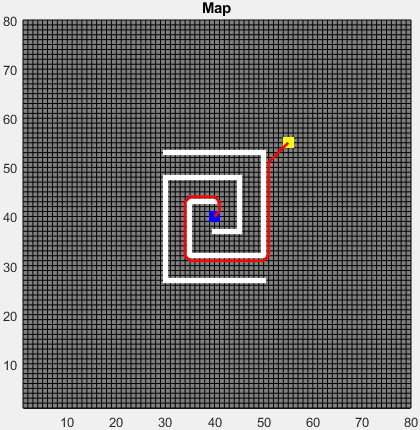
\includegraphics[width=\textwidth]{images/a_star_static_maze_1.png}
		\caption{Path taken by A* assuming static environment in maze 1.}
        \label{fig:a_star_static_path_maze_1}
	\end{subfigure}
    \hfill
	\begin{subfigure}[t]{0.32\columnwidth}
		\centering
		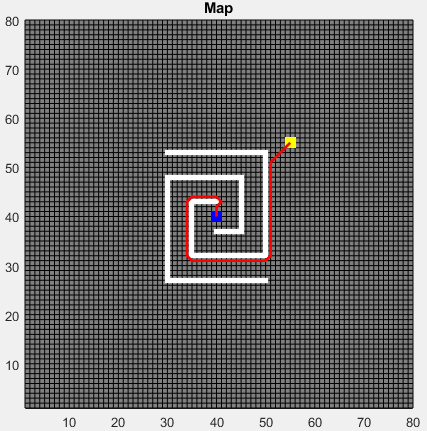
\includegraphics[width=\textwidth]{images/dijkstra_static_maze_1.png}
		\caption{Path taken by Dijkstra assuming static environment in maze 1.}
        \label{fig:dijkstra_static_path_maze_1}
	\end{subfigure}
    \hfill
    \begin{subfigure}[t]{0.32\columnwidth}
		\centering
		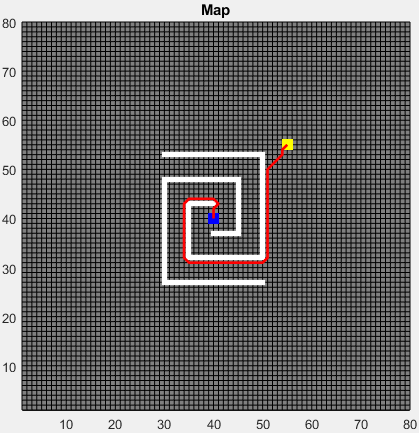
\includegraphics[width=\textwidth]{images/d_star_lite_static_maze_1.png}
		\caption{Path taken by D* lite assuming static environment in maze 1.}
        \label{fig:d_star_static_path_maze_1}
	\end{subfigure}
	\caption{Paths taken by all algorithms assuming static environment in maze 1.}
    \label{fig:static_path_maze_1}
\end{figure}

The evaluation measurements of all algorithms for static environment in maze 1 can be seen in Table.\:\ref{tab:metric_static_maze_1}.

\begin{table}
    \centering
    \begin{tabular}{c|c|c|c}
        Algorithm   & Pushes    & Pops      & Execution time (s)    \\ \hline
        A*          & $549$     & $503$     & $1.0489$              \\
        Dijkstra    & $3373$    & $3078$    & $37.2224$             \\
        D* lite     & $2805$    & $2524$    & $27.9366$
    \end{tabular}
    \caption{Evaluation measurements of all algorithms assuming static environment in maze 1.}
    \label{tab:metric_static_maze_1}
\end{table}

%-------------------------------------------------------------------------------------------
% Maze 2

Fig.\:\ref{fig:static_path_maze_2} presents the paths taken in static environment for maze 2. Fig.\:\ref{fig:a_star_static_path_maze_2} shows the path taken by A*, Dijkstra is shown in Fig.\:\ref{fig:dijkstra_static_path_maze_2}, and finally D* lite is shown in Fig.\:\ref{fig:d_star_static_path_maze_2}.

\begin{figure}
	\centering
    \begin{subfigure}[t]{0.32\columnwidth}
		\centering
		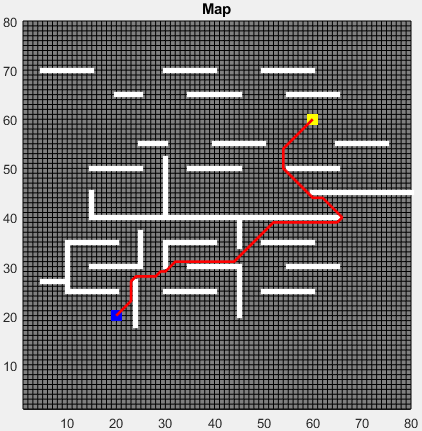
\includegraphics[width=\textwidth]{images/a_star_static_maze_2.png}
		\caption{Path taken by A* assuming static environment in maze 2.}
        \label{fig:a_star_static_path_maze_2}
	\end{subfigure}
    \hfill
	\begin{subfigure}[t]{0.32\columnwidth}
		\centering
		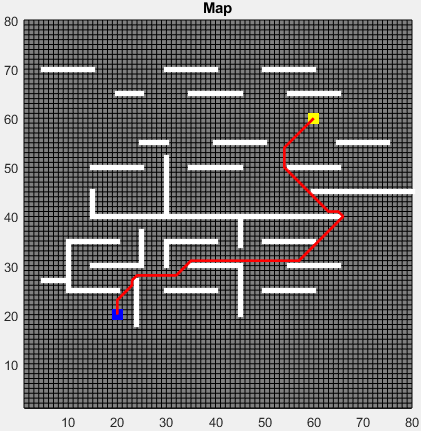
\includegraphics[width=\textwidth]{images/dijkstra_static_maze_2.png}
		\caption{Path taken by Dijkstra assuming static environment in maze 2.}
        \label{fig:dijkstra_static_path_maze_2}
	\end{subfigure}
    \hfill
    \begin{subfigure}[t]{0.32\columnwidth}
		\centering
		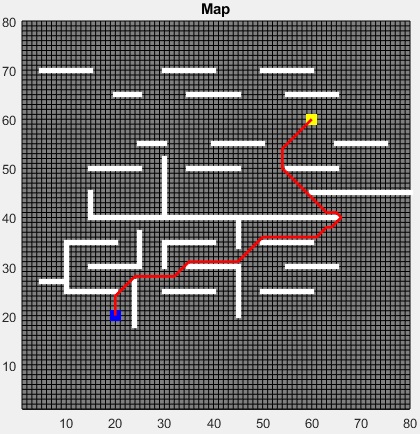
\includegraphics[width=\textwidth]{images/d_star_lite_static_maze_2.png}
		\caption{Path taken by D* lite assuming static environment in maze 2.}
        \label{fig:d_star_static_path_maze_2}
	\end{subfigure}
	\caption{Paths taken by all algorithms assuming static environment in maze 2.}
    \label{fig:static_path_maze_2}
\end{figure}

The evaluation measurements of all algorithms for static environment in maze 2 can be seen in Table.\:\ref{tab:metric_static_maze_2}.

\begin{table}
    \centering
    \begin{tabular}{c|c|c|c}
        Algorithm   & Pushes    & Pops      & Execution time (s)    \\ \hline
        A*          & $2649$    & $2440$    & $20.1303$             \\
        Dijkstra    & $5380$    & $5319$    & $38.893$              \\
        D* lite     & $2686$    & $2407$    & $19.5628$
    \end{tabular}
    \caption{Evaluation measurements of all algorithms assuming static environment in maze 2.}
    \label{tab:metric_static_maze_2}
\end{table}

%-------------------------------------------------------------------------------------------
% Maze 3

The paths taken through maze 3 by all the algorithms when the environment was static is shown in Fig.\:\ref{fig:static_path_maze_3}. Fig.\:\ref{fig:a_star_static_path_maze_3} shows the path taken by A*, Dijkstra is shown in Fig.\:\ref{fig:dijkstra_static_path_maze_3}, and finally D* lite is shown in Fig.\:\ref{fig:d_star_static_path_maze_3}.

\begin{figure}
	\centering
    \begin{subfigure}[t]{0.32\columnwidth}
		\centering
		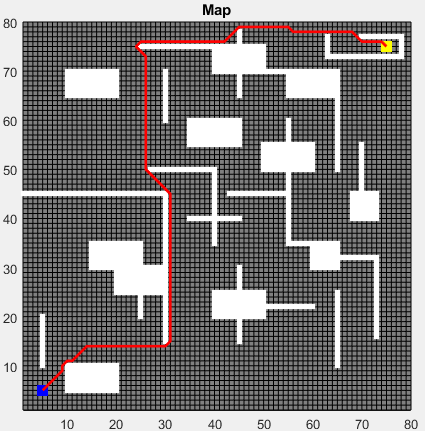
\includegraphics[width=\textwidth]{images/a_star_static_maze_3.png}
		\caption{Path taken by A* assuming static environment in maze 3.}
        \label{fig:a_star_static_path_maze_3}
	\end{subfigure}
    \hfill
	\begin{subfigure}[t]{0.32\columnwidth}
		\centering
		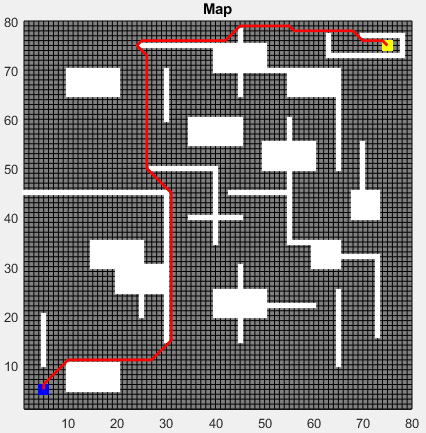
\includegraphics[width=\textwidth]{images/dijkstra_static_maze_3.png}
		\caption{Path taken by Dijkstra assuming static environment in maze 3.}
        \label{fig:dijkstra_static_path_maze_3}
	\end{subfigure}
    \hfill
    \begin{subfigure}[t]{0.32\columnwidth}
		\centering
		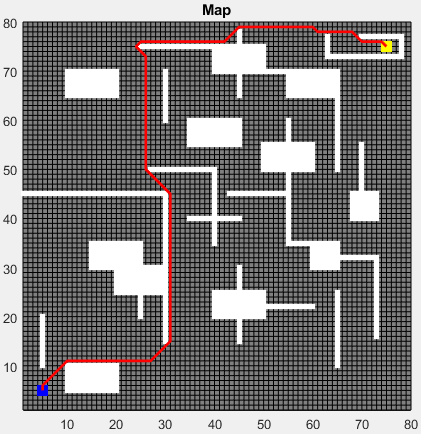
\includegraphics[width=\textwidth]{images/d_star_lite_static_maze_3.png}
		\caption{Path taken by D* lite assuming static environment in maze 3.}
        \label{fig:d_star_static_path_maze_3}
	\end{subfigure}
	\caption{Paths taken by all algorithms assuming static environment in maze 3.}
    \label{fig:static_path_maze_3}
\end{figure}

The evaluation measurements of all algorithms for static environment in maze 3 can be seen in Table.\:\ref{tab:metric_static_maze_3}.

\begin{table}
    \centering
    \begin{tabular}{c|c|c|c}
        Algorithm   & Pushes    & Pops      & Execution time (s)    \\ \hline
        A*          & $4953$    & $4873$    & $37.4206$             \\
        Dijkstra    & $5436$    & $5433$    & $30.7629$             \\
        D* lite     & $3348$    & $3181$    & $20.836$
    \end{tabular}
    \caption{Evaluation measurements of all algorithms assuming static environment in maze 3.}
    \label{tab:metric_static_maze_3}
\end{table}

%-------------------------------------------------------------------------------------------




%-------------------------------------------------------------------------------------------

\subsection{Dynamic environment}

%-------------------------------------------------------------------------------------------
% Maze 1

The paths taken by the algorithms when the environment was dynamic and maze 1 was used, can be seen in Fig.\:\ref{fig:dynamic_path_maze_1}. Fig.\:\ref{fig:a_star_dynamic_path_maze_1} shows the path taken by A*, Dijkstra is shown in Fig.\:\ref{fig:dijkstra_dynamic_path_maze_1}, and finally D* lite is shown in Fig.\:\ref{fig:d_star_dynamic_path_maze_1}.

\begin{figure}
	\centering
    \begin{subfigure}[t]{0.32\columnwidth}
		\centering
		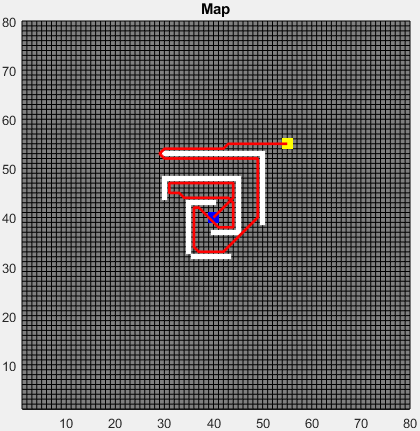
\includegraphics[width=\textwidth]{images/a_star_dynamic_maze_1.png}
		\caption{Path taken by A* assuming dynamic environment in maze 1.}
        \label{fig:a_star_dynamic_path_maze_1}
	\end{subfigure}
    \hfill
	\begin{subfigure}[t]{0.32\columnwidth}
		\centering
		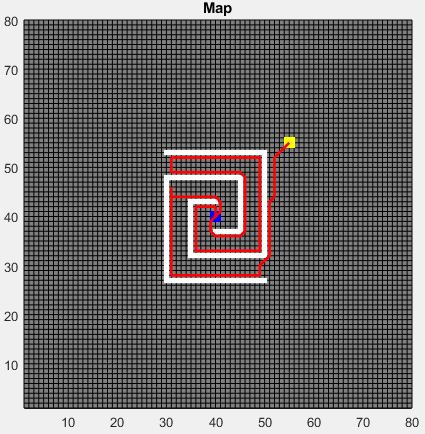
\includegraphics[width=\textwidth]{images/dijkstra_dynamic_maze_1.png}
		\caption{Path taken by Dijkstra assuming dynamic environment in maze 1.}
        \label{fig:dijkstra_dynamic_path_maze_1}
	\end{subfigure}
    \hfill
    \begin{subfigure}[t]{0.32\columnwidth}
		\centering
		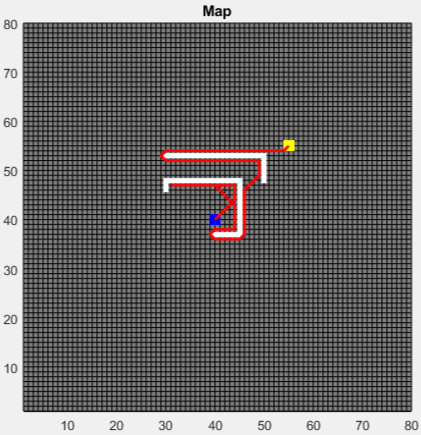
\includegraphics[width=\textwidth]{images/d_star_lite_dynamic_maze_1.png}
		\caption{Path taken by D* lite assuming dynamic environment in maze 1.}
        \label{fig:d_star_dynamic_path_maze_1}
	\end{subfigure}
	\caption{Paths taken by all algorithms assuming dynamic environment in maze 1.}
    \label{fig:dynamic_path_maze_1}
\end{figure}

The evaluation measurements of all algorithms for dynamic environment in maze 1 can be seen in Table.\:\ref{tab:metric_dynamic_maze_1}.

\begin{table}
    \centering
    \begin{tabular}{c|c|c|c}
        Algorithm   & Pushes    & Pops      & Execution time (s)    \\ \hline
        A*          & $2779$    & $1713$    & $2.7427$              \\
        Dijkstra    & $3683$    & $2468$    & $15.7218$             \\
        D* lite     & $1206$    & $1031$    & $7.9151$
    \end{tabular}
    \caption{Evaluation measurements of all algorithms assuming dynamic environment in maze 1.}
    \label{tab:metric_dynamic_maze_1}
\end{table}

%-------------------------------------------------------------------------------------------
% Maze 2

The paths taken through maze 2 when the environment was dynamic, can be seen in Fig.\:\ref{fig:dynamic_path_maze_2}. Fig.\:\ref{fig:a_star_dynamic_path_maze_2} shows the path taken by A*, Dijkstra is shown in Fig.\:\ref{fig:dijkstra_dynamic_path_maze_2}, and finally D* lite is shown in Fig.\:\ref{fig:d_star_dynamic_path_maze_2}.

\begin{figure}
	\centering
    \begin{subfigure}[t]{0.32\columnwidth}
		\centering
		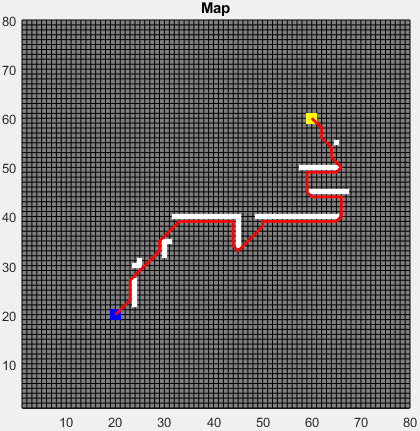
\includegraphics[width=\textwidth]{images/a_star_dynamic_maze_2.png}
		\caption{Path taken by A* assuming dynamic environment in maze 2.}
        \label{fig:a_star_dynamic_path_maze_2}
	\end{subfigure}
    \hfill
	\begin{subfigure}[t]{0.32\columnwidth}
		\centering
		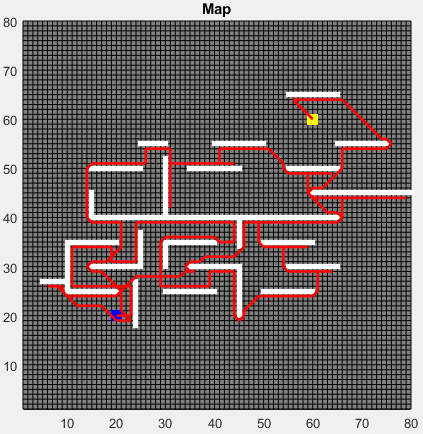
\includegraphics[width=\textwidth]{images/dijkstra_dynamic_maze_2.png}
		\caption{Path taken by Dijkstra assuming dynamic environment in maze 2.}
        \label{fig:dijkstra_dynamic_path_maze_2}
	\end{subfigure}
    \hfill
    \begin{subfigure}[t]{0.32\columnwidth}
		\centering
		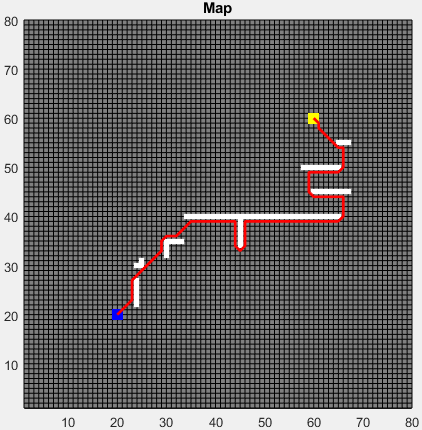
\includegraphics[width=\textwidth]{images/d_star_lite_dynamic_maze_2.png}
		\caption{Path taken by D* lite assuming dynamic environment in maze 2.}
        \label{fig:d_star_dynamic_path_maze_2}
	\end{subfigure}
	\caption{Paths taken by all algorithms assuming dynamic environment in maze 2.}
    \label{fig:dynamic_path_maze_2}
\end{figure}

The evaluation measurements of all algorithms for dynamic environment in maze 2 can be seen in Table.\:\ref{tab:metric_dynamic_maze_2}.

\begin{table}
    \centering
    \begin{tabular}{c|c|c|c}
        Algorithm   & Pushes    & Pops      & Execution time (s)    \\ \hline
        A*          & $693$     & $229$     & $0.27295$             \\
        Dijkstra    & $11858$   & $8532$    & $41.4283$             \\
        D* lite     & $1170$    & $904$     & $11.811$
    \end{tabular}
    \caption{Evaluation measurements of all algorithms assuming dynamic environment in maze 2.}
    \label{tab:metric_dynamic_maze_2}
\end{table}

%-------------------------------------------------------------------------------------------
% Maze 3

Fig.\:\ref{fig:dynamic_path_maze_3} presents the paths taken through maze 3 by all algorithms when the environment was dynamic. Fig.\:\ref{fig:a_star_dynamic_path_maze_3} shows the path taken by A*, Dijkstra is shown in Fig.\:\ref{fig:dijkstra_dynamic_path_maze_3}, and finally D* lite is shown in Fig.\:\ref{fig:d_star_dynamic_path_maze_3}.

\begin{figure}
	\centering
    \begin{subfigure}[t]{0.32\columnwidth}
		\centering
		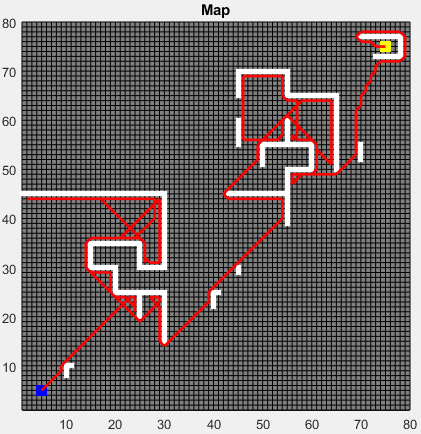
\includegraphics[width=\textwidth]{images/a_star_dynamic_maze_3.png}
		\caption{Path taken by A* assuming dynamic environment in maze 3.}
        \label{fig:a_star_dynamic_path_maze_3}
	\end{subfigure}
    \hfill
	\begin{subfigure}[t]{0.32\columnwidth}
		\centering
		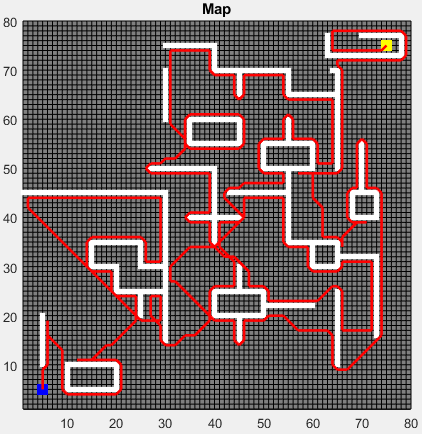
\includegraphics[width=\textwidth]{images/dijkstra_dynamic_maze_3.png}
		\caption{Path taken by Dijkstra assuming dynamic environment in maze 3.}
        \label{fig:dijkstra_dynamic_path_maze_3}
	\end{subfigure}
    \hfill
    \begin{subfigure}[t]{0.32\columnwidth}
		\centering
		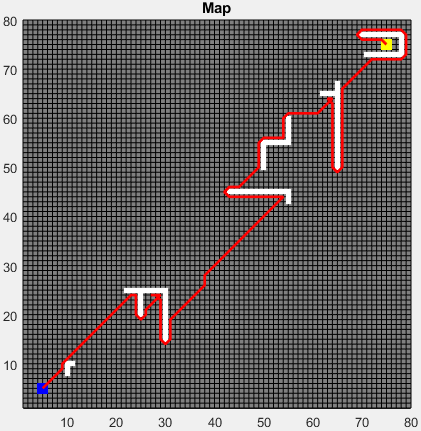
\includegraphics[width=\textwidth]{images/d_star_lite_dynamic_maze_3.png}
		\caption{Path taken by D* lite assuming dynamic environment in maze 3.}
        \label{fig:d_star_dynamic_path_maze_3}
	\end{subfigure}
	\caption{Paths taken by all algorithms assuming dynamic environment in maze 3.}
    \label{fig:dynamic_path_maze_3}
\end{figure}

The evaluation measurements of all algorithms for dynamic environment in maze 3 can be seen in Table.\:\ref{tab:metric_dynamic_maze_3}.

\begin{table}
    \centering
    \begin{tabular}{c|c|c|c}
        Algorithm   & Pushes    & Pops      & Execution time (s)    \\ \hline
        A*          & $7210$    & $4356$    & $7.5347$              \\
        Dijkstra    & $14634$   & $9867$    & $31.382$              \\
        D* lite     & $2593$    & $2155$    & $47.4293$
    \end{tabular}
    \caption{Evaluation measurements of all algorithms assuming dynamic environment in maze 3.}
    \label{tab:metric_dynamic_maze_3}
\end{table}

%-------------------------------------------------------------------------------------------
\section{Discussion}
%-------------------------------------------------------------------------------------------
% A small discussion on the result

% A*
The results indicate that A* is the most efficient algorithm in small static environments, but the overhead clearly limits the algorithm in large environments where the algorithm approaches Dijkstra's efficiency. A* is the most efficient in terms of execution time in dynamic environments of all sizes, a surprising result given that it has poor execution time in large static environments.
% Dijkstra
Dijkstra performs the worst in all test scenarios (except execution time in largest map in unknown environments), clearly showing its inefficiency compared to the other algorithms. The paths produced by Dijkstra in dynamic environments is also very non optimal. Dijkstra mainly performs poorly in terms of pushes and pops, always searching substantially larger spaces than both A* and D* lite. 
% D* lite
D* lite has very favorable results in larger environments, especially dynamic, when it comes to pushes and pops. The poor execution time could be the result of the implementation not being optimized. The results also show that D* lite finds more optimized paths in dynamic environments, compared to A* and Dijkstra.

%-------------------------------------------------------------------------------------------
%\section{Conclusion}
%\section*{Acknowledgment}

% Select the IEEEtran style
\bibliographystyle{IEEEtran}
% Include bibliography file
\bibliography{refs,ELA408_Path}
\end{document}